% Created 2022-03-30 Wed 04:01
% Intended LaTeX compiler: pdflatex
\documentclass[11pt]{article}
\usepackage[utf8]{inputenc}
\usepackage[T1]{fontenc}
\usepackage{graphicx}
\usepackage{longtable}
\usepackage{wrapfig}
\usepackage{rotating}
\usepackage[normalem]{ulem}
\usepackage{amsmath}
\usepackage{amssymb}
\usepackage{capt-of}
\usepackage{hyperref}
\usepackage[margin=0.5in]{geometry}
\author{Marc Soda Jr}
\date{\today}
\title{CSE-343 | Firewall Exploration Lab}
\hypersetup{
 pdfauthor={Marc Soda Jr},
 pdftitle={CSE-343 | Firewall Exploration Lab},
 pdfkeywords={},
 pdfsubject={},
 pdfcreator={Emacs 27.2 (Org mode 9.5.2)},
 pdflang={English}}
\begin{document}

\maketitle
\tableofcontents

\section*{Task 1.A:}
\label{sec:org7c924fe}
\begin{itemize}
\item I followed the instructions as specified in the PDF and was successful. The only difference was that I added `MODULE\textsubscript{LICENSE}("GPL");` to hello.c because I got a make error because the license was not specified.
\item Code:
\begin{center}
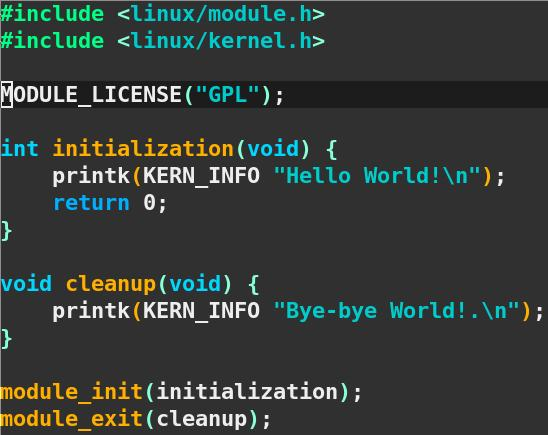
\includegraphics[width=.9\linewidth]{./images/00.jpg}
\end{center}
\item dmesg output:
\begin{center}
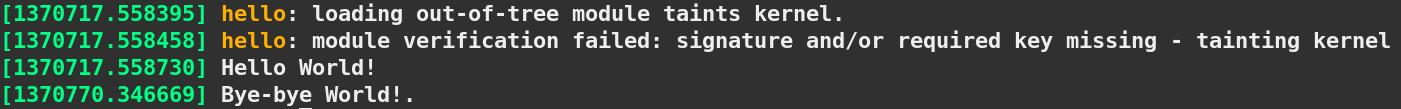
\includegraphics[width=.9\linewidth]{./images/01.jpg}
\end{center}
\end{itemize}
\section*{Task 1.B:}
\label{sec:org22ae1d9}
\subsection*{Task 1:}
\label{sec:org548b5dd}
\begin{itemize}
\item Before adding the module, I am able to dig google.com with no issue. After adding the module, the request is blocked.
\item Proof:
\begin{center}
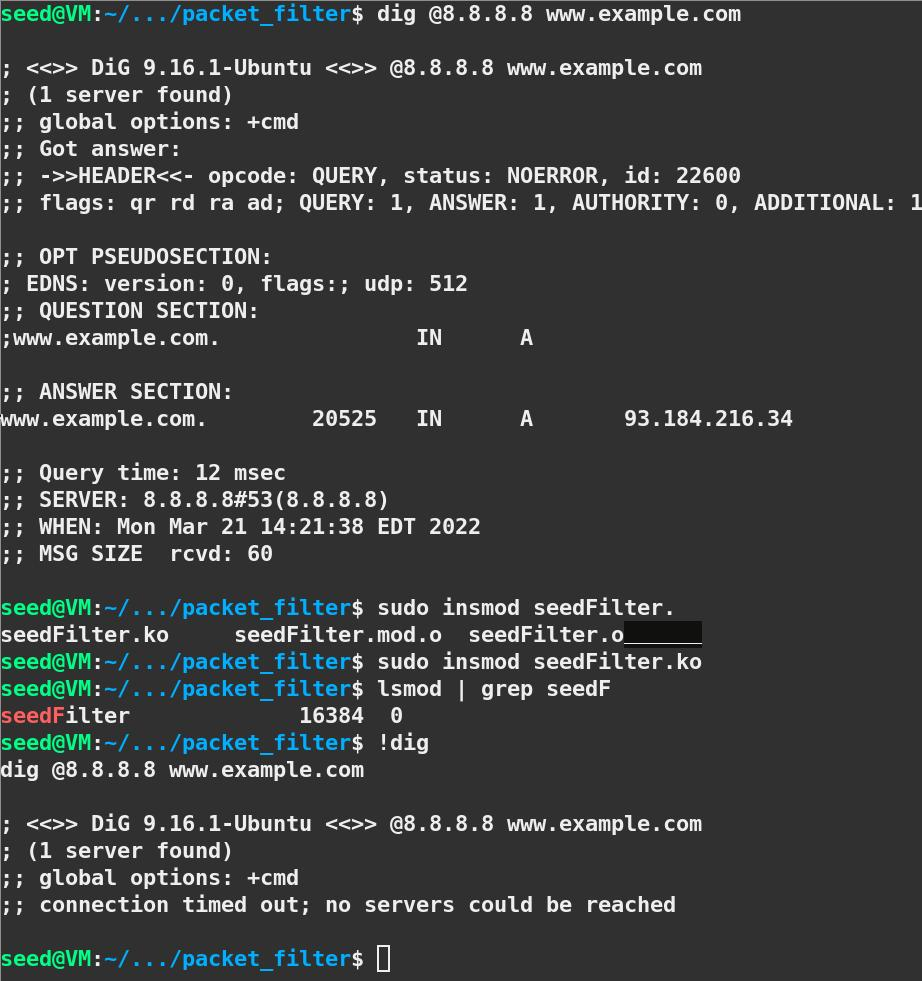
\includegraphics[width=.9\linewidth]{./images/02.jpg}
\end{center}
\end{itemize}
\subsection*{Task 2:}
\label{sec:org1e7d050}
\begin{itemize}
\item Code
\begin{center}
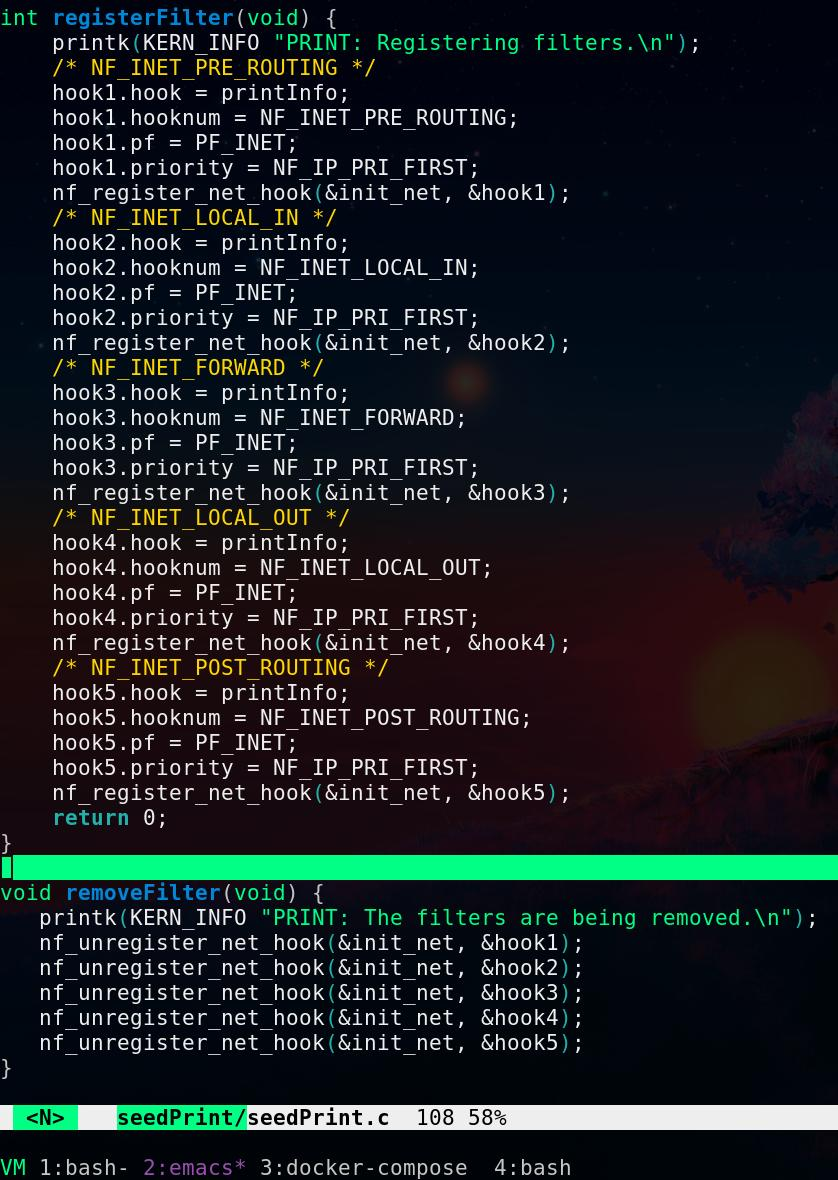
\includegraphics[width=.9\linewidth]{./images/03.jpg}
\end{center}
\item After adding the module, I can the information being printed (through dmesg) corresponding to each hook.
\begin{center}
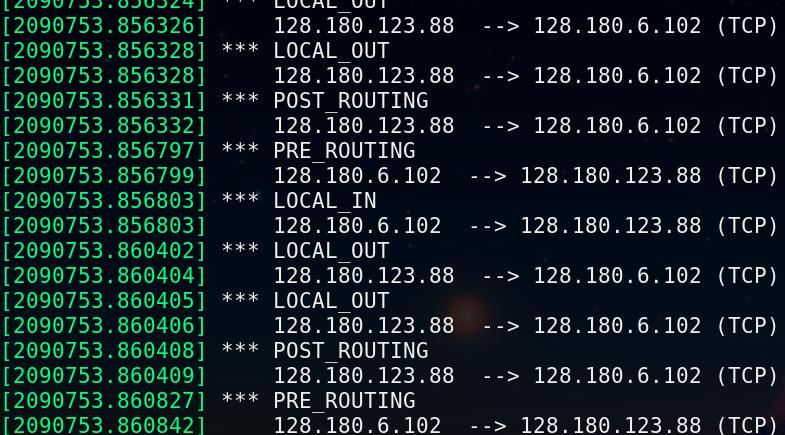
\includegraphics[width=.9\linewidth]{./images/04.jpg}
\end{center}
\end{itemize}
\subsection*{Task 3:}
\label{sec:orge2d9147}
\begin{itemize}
\item blockPing and blockTelnet code:
\begin{center}
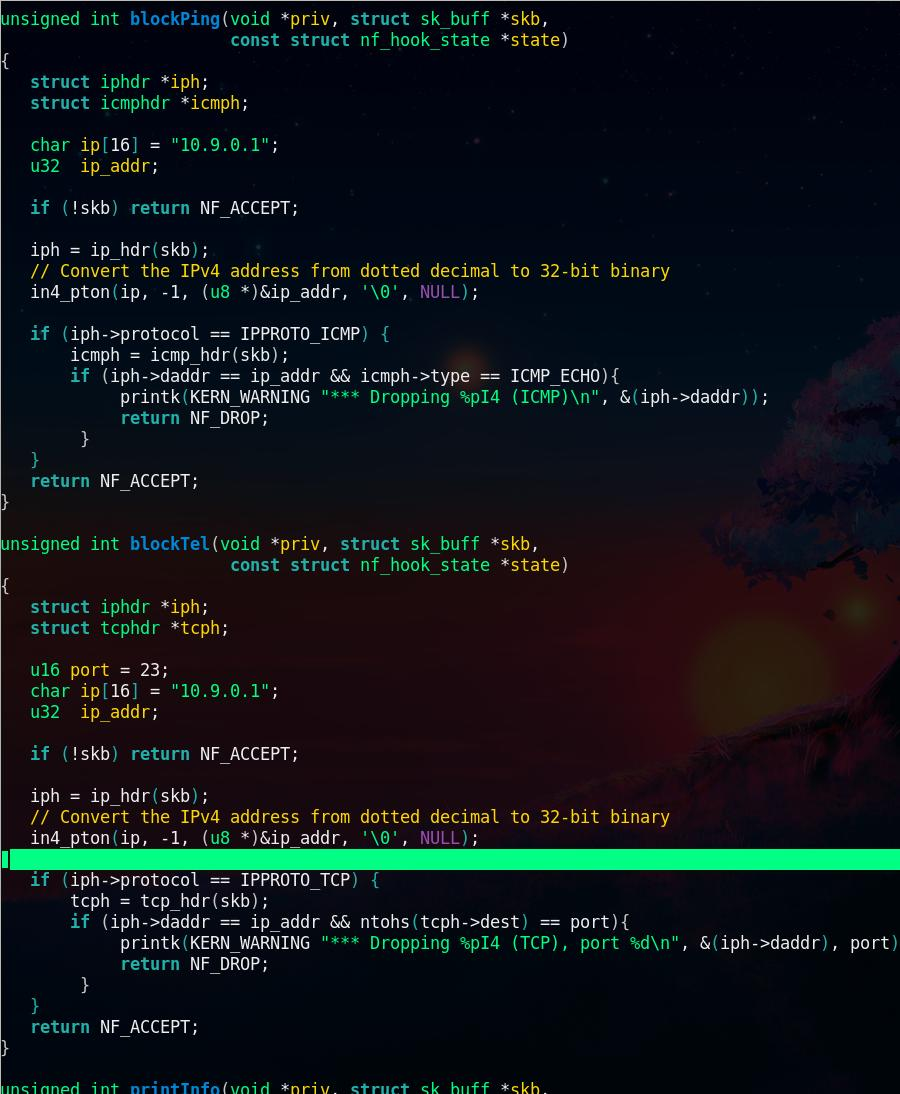
\includegraphics[width=.9\linewidth]{./images/06.jpg}
\end{center}
\item The following screenshot shows two shells. One shows HostA running telnet and ping. The other is a filtered cat of syslog showing which packets were dropped as a result of this task. As you can see, the new kernel module is blocking telnet and icmp packets. The reason why I could not show dmesg output is because when I do `dmesg -k -w`, the output scrolls much too fast to read. I believe this is because I am connected to my seed server over ssh.
\begin{center}
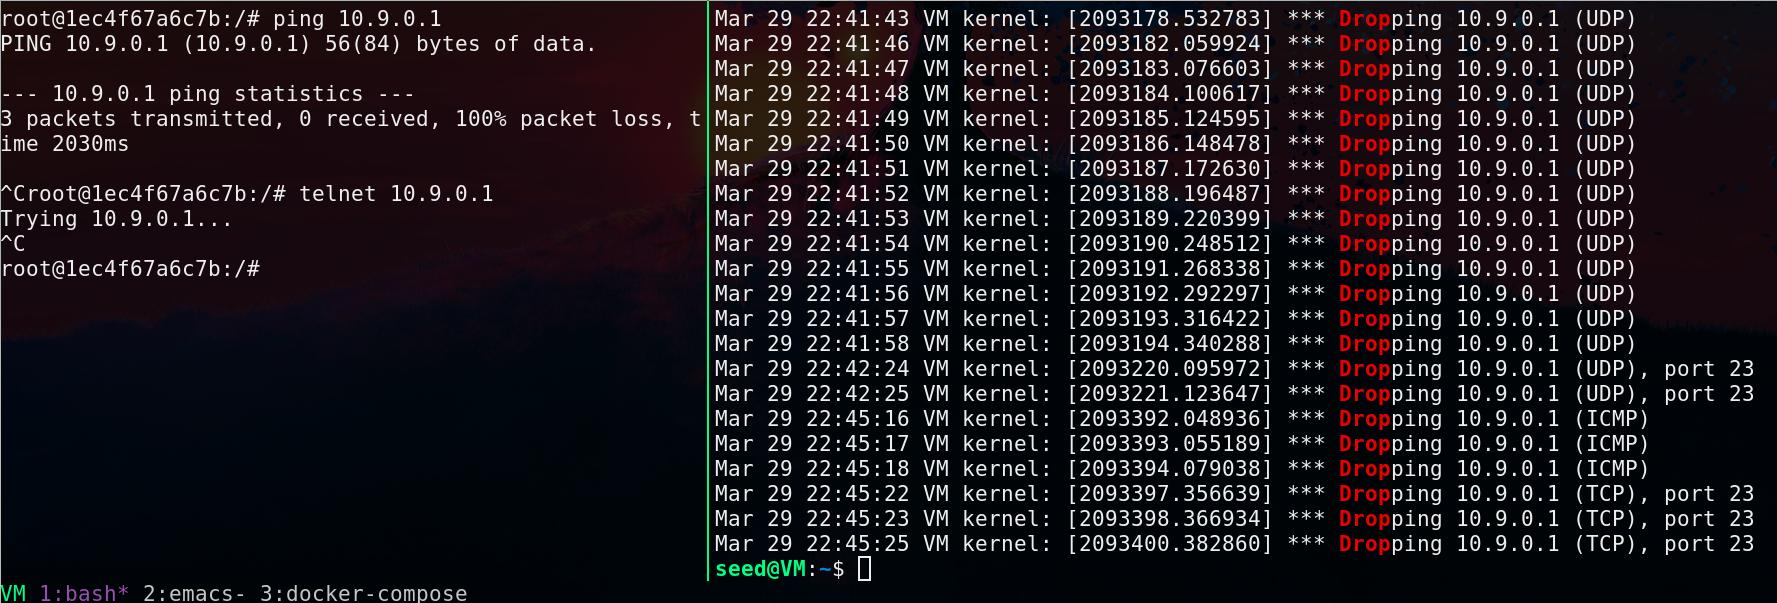
\includegraphics[width=.9\linewidth]{./images/05.jpg}
\end{center}
\end{itemize}

\section*{Task 2:}
\label{sec:org147855f}
\subsection*{Task 2A:}
\label{sec:orgbc64358}
\begin{itemize}
\item Before manipulating the IP tables I can ping and telnet into the router (10.9.0.11) just fine.
\item After manipulating the IP tables with the specified command, I can ping the router, but I can't telnet into it.
\item These rules drop ICMP packets except for PING.
\end{itemize}
\subsection*{Task 2B:}
\label{sec:org10b1335}
\begin{itemize}
\item Commands (see screenshot for iptables rules output):
\begin{itemize}
\item iptables -A FORWARD -i eth0 -p icmp --icmp-type echo-request -j DROP
\item iptables -A FORWARD -i eth1 -p icmp --icmp-type echo-request -j ACCEPT
\item iptables -A FORWARD -i eth0 -p icmp --icmp-type echo-reply -j ACCEPT
\item iptables -P FORWARD DROP
\end{itemize}
\item Observations (see screenshot for proof):
\begin{itemize}
\item HostA (outside) cannot ping Host1 (inside).
\item HostA (outside) can ping the router.
\item HostA (outside) cannot telnet Host1 (inside).
\item Host1 (inside) can ping HostA (outside)
\item Host1 (inside) cannot telnet HostA (outside)
\end{itemize}
\item Screenshot
\begin{itemize}
\item Top right is Host1. Bottom left is router. Bottom right is HostA. Hostnames reflected in prompt.
\begin{center}
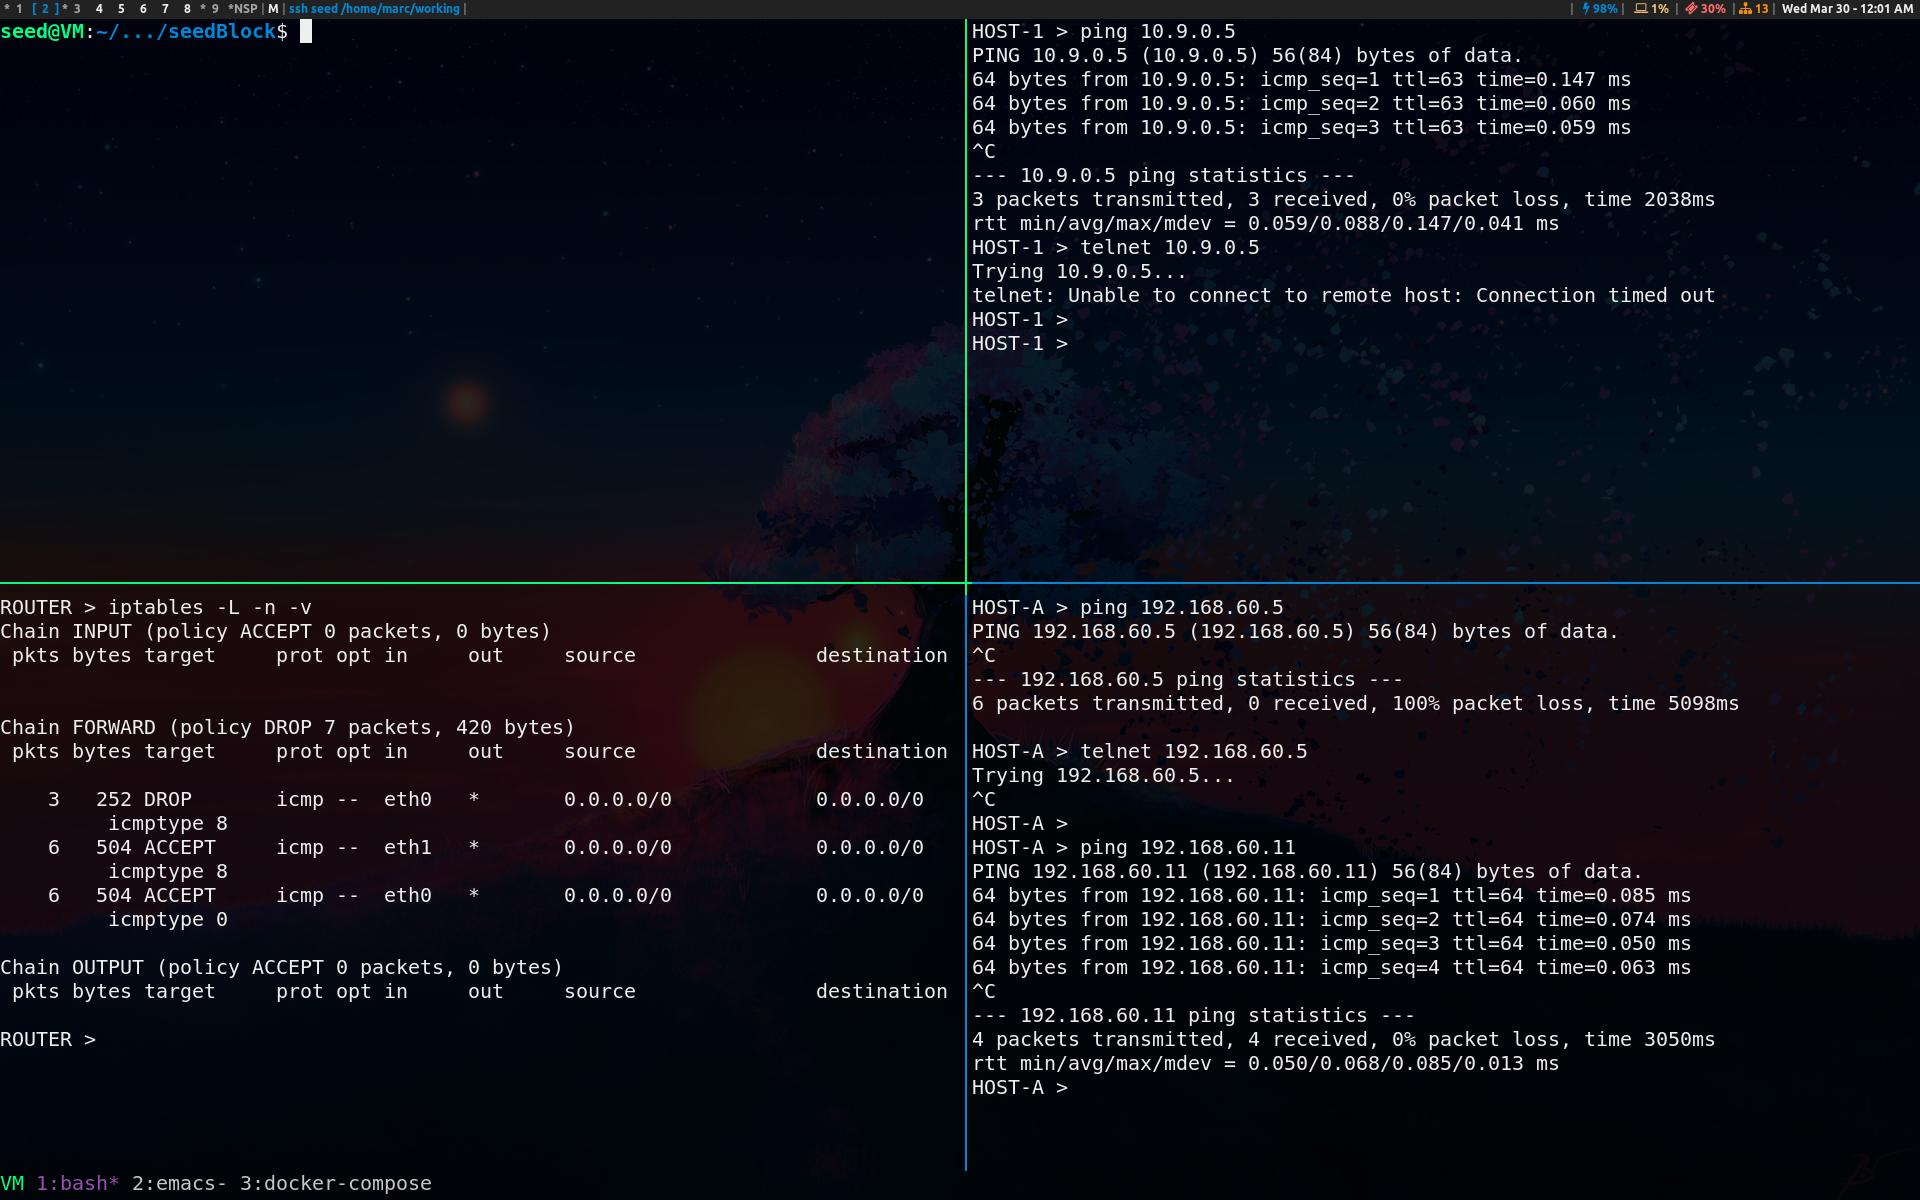
\includegraphics[width=.9\linewidth]{./images/07.jpg}
\end{center}
\end{itemize}
\end{itemize}
\subsection*{Task 2C:}
\label{sec:org864d75f}
\begin{itemize}
\item Commands (see screenshot for iptables rules output)
\begin{itemize}
\item iptables -A FORWARD -i eth0 -p tcp -d 192.160.60.5 --dport 23 -j ACCEPT
\item iptables -A FORWARD -i eth1 -p tcp -s 192.160.60.5 --sport 23 -j ACCEPT
\item iptables -P FORWARD DROP
\item iptables -A FORWARD -i eth0 -p tcp -sport 5000 -j ACCEPT
\end{itemize}
\item Observations (see screenshot for proof)
\begin{itemize}
\item Host1 (inside) is able to telnet into other hosts on the internal network.
\item HostA (outside) is able to telnet to Host1 (inside), but not to any other internal hosts.
\item Host1 (inside) is unable to telnet to HostA (outside).
\item Note that other internal and external hosts were tested and the specifications were met. See screenshot.
\end{itemize}
\end{itemize}
\begin{center}
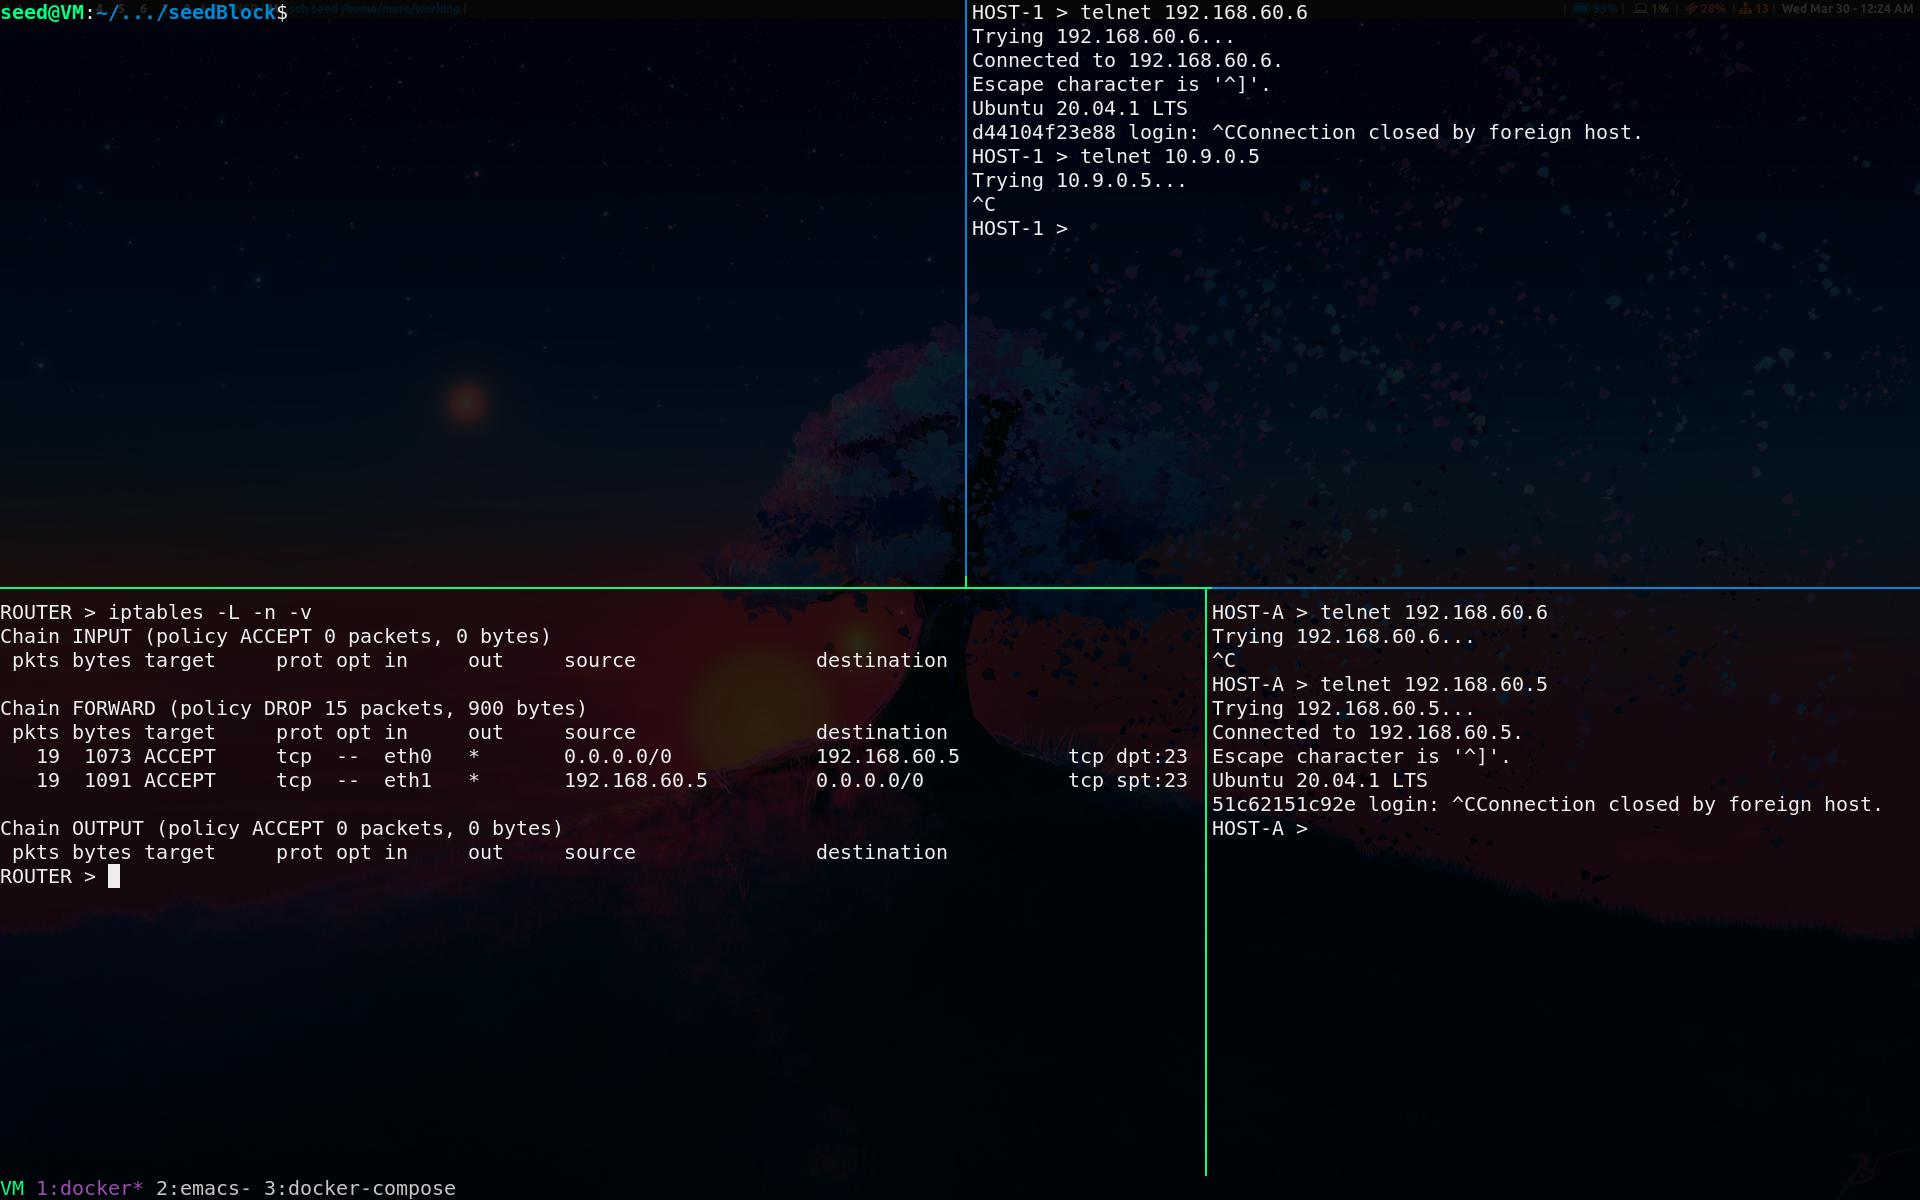
\includegraphics[width=.9\linewidth]{./images/08.jpg}
\end{center}
\section*{Task 3:}
\label{sec:orgc11818a}
\subsection*{Task 3A:}
\label{sec:org26e9fd5}
\subsubsection*{ICMP Experiment:}
\label{sec:org6531321}
\begin{itemize}
\item After pinging Host1 from the router, conntrack -L shows details about the connection that was made.
\item The ICMP connection state was kept for 30 seconds.
\end{itemize}
\subsubsection*{UDP Experiment:}
\label{sec:org29713bd}
\begin{itemize}
\item After communicating to Host1 from the router, conntrack -L shows details about the connection that was made.
\item The UDP connection state was kept for 30 seconds.
\end{itemize}
\subsubsection*{TCP Experiment:}
\label{sec:org217831f}
\begin{itemize}
\item After communicating from Host1 from the router, conntrack -L shows details about the connection that was made.
\item The TCP connection state was kept for 120 seconds.
\end{itemize}
\subsection*{Task 3B:}
\label{sec:org53765da}
\subsubsection*{Commands:}
\label{sec:org79ab2a2}
\begin{itemize}
\item iptables -A FORWARD -p tcp -i eth0 -d 192.168.60.5 --dport 23 --syn -m conntrack --ctstate NEW -j ACCEPT
\item iptables -A FORWARD -p tcp -i eth1 --syn -m conntrack --ctstate NEW -j ACCEPT
\item iptables -A FORWARD -p tcp -m conntrack --ctstate ESTABLISHED,RELATED -j ACCEPT
\item iptables -A FORWARD -p tcp -j DROP
\item iptables -A FORWARD ACCEPT
\end{itemize}
\subsubsection*{Observations (see screenshot):}
\label{sec:orge8a8a2b}
\begin{itemize}
\item HostA (outside) can telnet to Host1 (inside)
\item Host1 (inside) can telnet to HostA (outside)
\item These patterns are maintained for other internal and external hosts.
\end{itemize}
\begin{center}
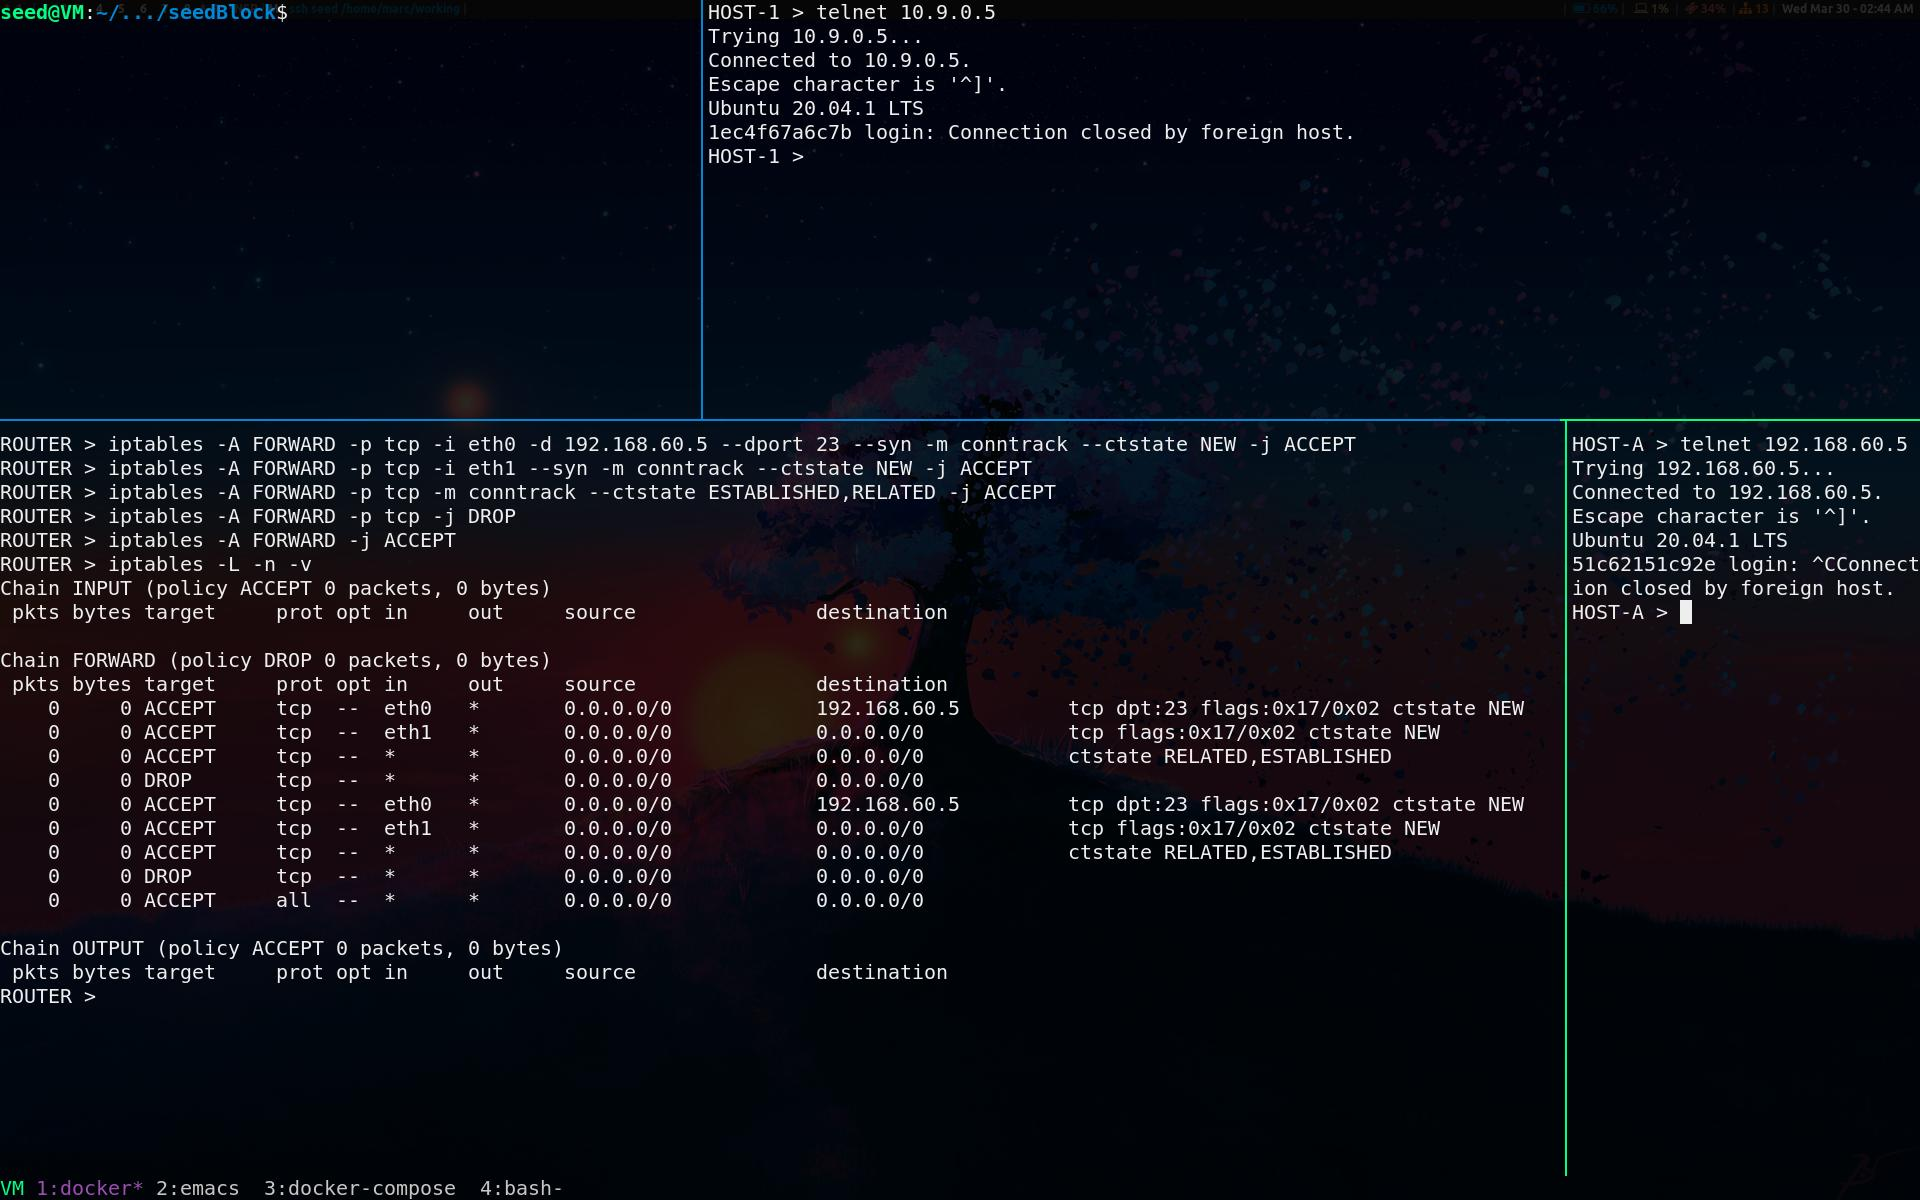
\includegraphics[width=.9\linewidth]{./images/09.jpg}
\end{center}
\subsubsection*{Conntrack advantages:}
\label{sec:orgc6da0ea}
\begin{itemize}
\item Consumes less CPU because caching
\end{itemize}
\subsubsection*{Conntrack disadvantages:}
\label{sec:org42f3293}
\begin{itemize}
\item Consumes more memory because connection states need to be saved for a certain amount of time.
\item Can be poor at handling a high volume of connections per second.
\end{itemize}
\section*{Task 4:}
\label{sec:org1442e4a}
\begin{itemize}
\item After running the first command only, pinging 192.168.60.5 is unaffected.
\item After adding the second rule, the following behavior is observed:
\begin{itemize}
\item The first 5 pings go through as normal.
\item Pings then begin being blocked due to the 5 connection burst limit and the 10/minute limit. I ended up getting a 67\% packet loss after 10 successful pings.
\end{itemize}
\end{itemize}
\section*{Task 5:}
\label{sec:org9091d47}
\subsection*{Round Robin Mode}
\label{sec:orga032260}
\subsubsection*{Commands:}
\label{sec:orga2de8c5}
\begin{itemize}
\item iptables -t nat -A PREROUTING -p udp --dport 8080 -m statistic --mode nth --every 3 --packet 0 -j DNAT --to-destination 192.168.60.5:8080
\item iptables -t nat -A PREROUTING -p udp --dport 8080 -m statistic --mode nth --every 2 --packet 0 -j DNAT --to-destination 192.168.60.6:8080
\item iptables -t nat -A PREROUTING -p udp --dport 8080 -m statistic --mode nth --every 1 --packet 0 -j DNAT --to-destination 192.168.60.7:8080
\item Each rule chooses which number packet (out of three) to send to each different server.
\end{itemize}
\subsubsection*{Observations}
\label{sec:orgc1246ed}
\begin{itemize}
\item After adding the rules, I can make a connection and send a message from HostA to the router. Each time a connection is made, it is forwarded to a different server on the network. First Host1, then Host2, then Host3, then repeat. The load balancing task was successful. See screenshot.
\end{itemize}
\begin{center}
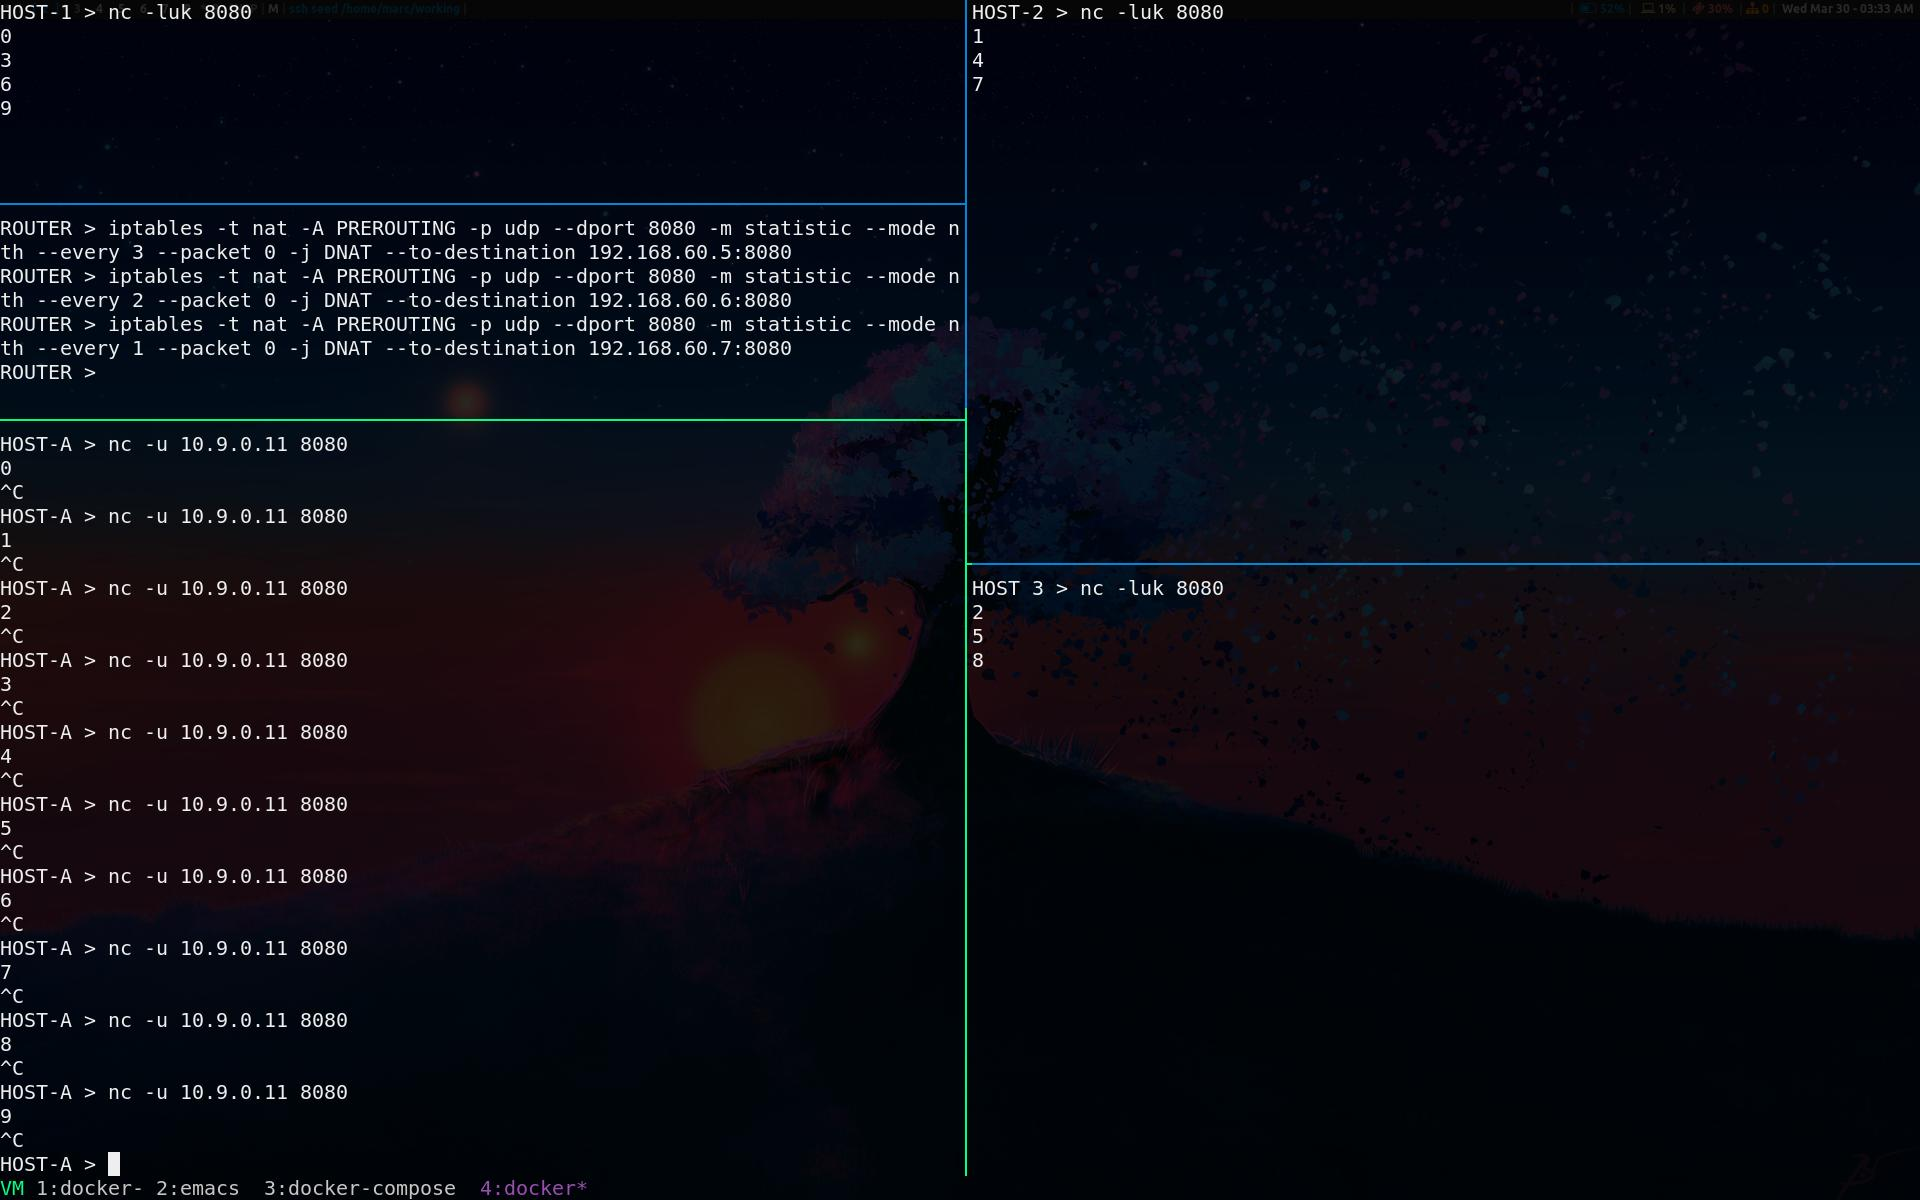
\includegraphics[width=.9\linewidth]{./images/10.jpg}
\end{center}
\subsection*{Random Mode}
\label{sec:org864f283}
\subsubsection*{Commands}
\label{sec:org758e6e9}
\begin{itemize}
\item iptables -t nat -A PREROUTING -p udp --dport 8080 -m statistic --mode random --probability .3333 -j DNAT --to-destination 192.168.60.5:8080
\item iptables -t nat -A PREROUTING -p udp --dport 8080 -m statistic --mode random --probability .5 -j DNAT --to-destination 192.168.60.6:8080
\item iptables -t nat -A PREROUTING -p udp --dport 8080 -m statistic --mode random --probability 1 -j DNAT --to-destination 192.168.60.7:8080
\item Apparently making the probability for each rule .3333 is wrong. When I did that I found that the connection would get dropped sometimes. I had to look it up and apparently you are supposed to make the first one .3333, the second .5, and the third 1. This has something to do with the fact that the rules are executed sequentially. With this setup, each host has a 33\% chance of being selected.
\end{itemize}
\subsubsection*{Observations}
\label{sec:orgfd3df05}
\begin{center}
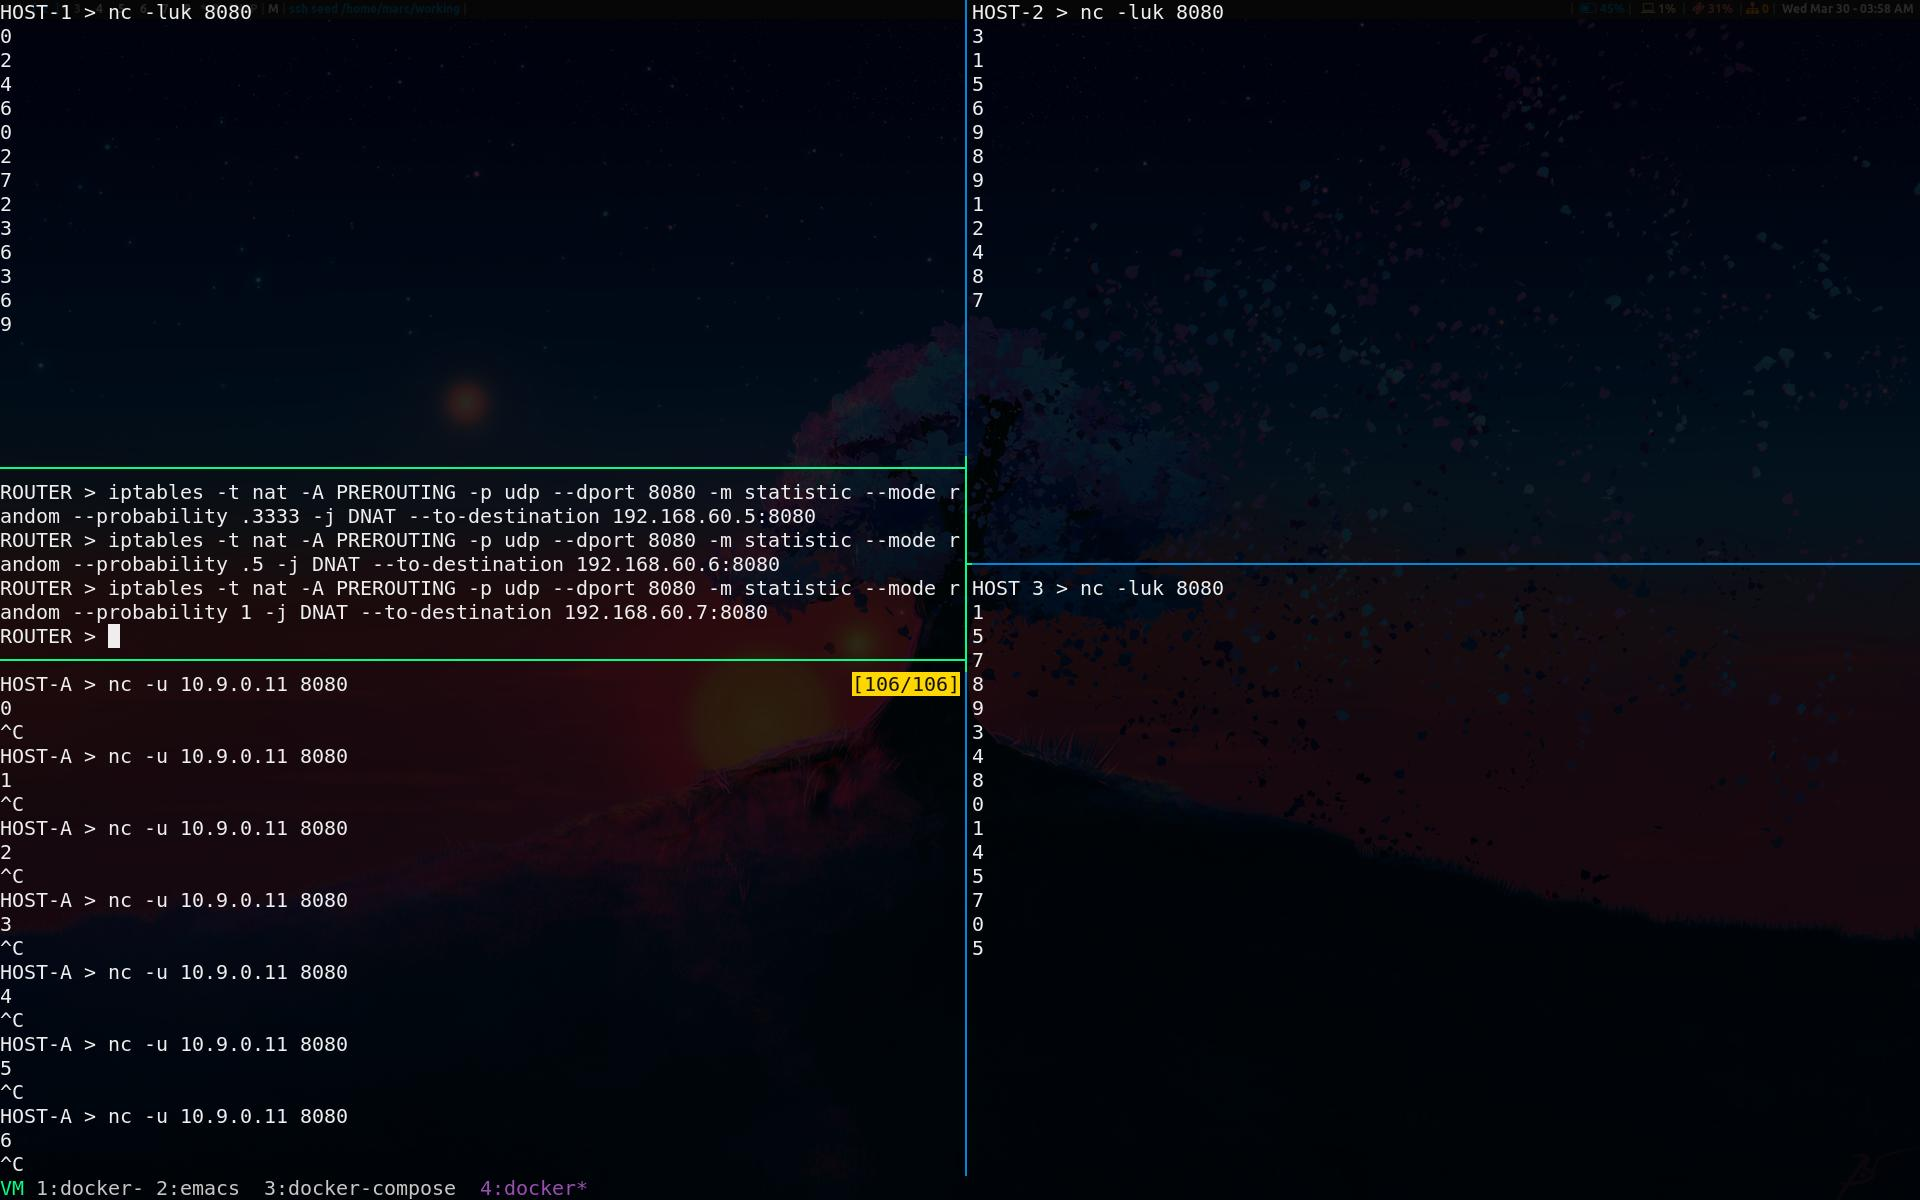
\includegraphics[width=.9\linewidth]{./images/11.jpg}
\end{center}
\end{document}